\chapter{Background}
Accidental falls and accidents resulting in injury is a large scale world wide problem, A study conducted by the American Journal of Public Health found that one of the leading causes of death is falling, for people aged 50 or above , a 136\% increase over a 30 year period\cite{fallDeaths}.  Accidents are not aged biased however certain sports come with a higher probability of accidents occuring.
Like all extreme sports, mountain biking comes with the potential for serious injury to the rider in the event of an accident. In 2018 there were 29,000+ registered members of cycling Ireland in over 450 clubs \cite{IT1} , with this number set to increase year on year. With an increase of the number of people taking up the sport, the amount of reported injuries has also increased significantly.  A study conducted by Paracelsus Medical University recorded injury rates as high as 16.8 injuries per 1000 hours of riding, with 22\% being moderate and 16\% being severe \cite{studyOfMTBInjuries}. The most common mechanism of acute severe injury for mountain bikers has been found to be  falling forward (64.9\%), which lead to the most severe injuries, with an ISS \footnote{ Injury Severity Score} of 3.4 out of a possible 6 (currently untreatable ) \cite{InjuryScale}


Existing solutions for fall detection for both medical (Fall detection for the elderly) as well as existing crash detection systems for cyclists will be discussed and explained in this chapter.

\newpage
\section{The Concept}

Fall detection for the elderly has been around for decades, the original idea came to fruition as a result of the impracticality of having around the clock care for the independent, but fragile members of society. With high success rates and the advancement of technology in recent years the concept has been applied to many different uses cases, such as accident detection in vehicles and sports. 


\section{Existing Solutions - Medical}
Fall detection is not a new concept in the medical domain, The first fall monitoring system (PERS\footnote{Personal Emergency Response System}) Hausnotruf  was developed in the 1970’s by Wilhelm Hormann  These early active systems were manually triggered, requiring the user to activate them by pressing a button on a transceiver, while relying on an active phone line in the home to contact help. Active systems have been mostly phazed out due to their main weakness - the user must be conscious and capable of triggering the alarm. Passive systems are now commonplace and most relevant to this study. Passive systems monitor the users movement and trigger the alarm without the need for user interaction with the system. Passive systems can be implemented in one of two ways: Vision Based approaches and wearable sensor based solutions. Currently Sensor based solutions are widely available, while computer vision implementations are mostly experimental proof of concepts.  


\subsection{Vision Based Approaches}
Computer Vision Approaches are currently the state of the art in terms of fall detection for the elderly, these systems comprise of multiple cameras set up in the home, with a base station analysing the video footage to determine if the user is in need of assistance. Implementing Computer Vision techniques such as optical flow or Gaussian Mixture Models, to focus on moving objects and ignoring the background, allows for recognition of falls or slips. Many environmental issues such as changing lighting and limited view of cameras in the home impede the accuracy of these systems. Unfortunately for these systems it is not possible to constrain the environment enough to allow for near perfect accuracy.
Vision based approaches also pose a large risk to the occupants privacy. 24/7 surveillance in the home is not something anyone desires, especially in what is supposed to be the comfort of your own home. Depending on the security utilized, vulnerabilities may exist exposing the stream to the world.

Cost is a large factor in why sensor based solutions are prefered, the cost of initial setup is much higher for a computer vision solution. Adding complexity to an implementation while simple more effective solutions, with similar or in some cases better results is a step in the wrong direction for now, however as technology further improves vision solutions will be more viable to bring to market.

\vspace{3cm}
\subsection{Sensor Based Approaches}
Wearable sensor based solutions are very common globally, in both passive and active products. These wearable devices are usually in the form of a small external device.

These devices can be:
\begin{itemize}
\item Wrist mounted
\item Attached to a belt
\item A Pendant worn around the neck.
\end{itemize}

Housed within these enclosures are embedded sensors, the most common of which is the triaxial accelerometer. The triaxial accelerometer measures proper acceleration in 3 perpendicular axis (g-force). Almost every wearable fall detector factors in accelerometer values while determining if a fall has occurred or not. The second most common sensor used in fall detection is the triaxial gyroscope, used to calculate rotational speed. Gyroscopes have proven to be useful for understanding the direction of a fall. Depending on where the device is worn, some false positives which would occur using only an accelerometer can be disregarded, such as sitting down too quickly. A pendant style device’s relative rotation would be more or less unchanged sitting down vs standing. The use of highly sensitive barometric sensors have also been utilized to measure minute changes in atmospheric pressure, the difference between pressure when one is standing vs lying down can be distinguished between. The most popular commercially available fall detection using barometric sensors is lifeline \cite{lifeline}. There is no standard passive implementation, solutions include one or more of the above sensors along with an algorithm or formula to determine if a fall has occurred. A comparison of sensors most commonly used can be seen in Table \ref{sen}.

\begin{table}
\caption{Comparison Of Sensors Used In Existing Solutions}
\label{sen}
\begin{center}

 \begin{tabular}{||c| c| c|  c| c| c||} 

 \hline
 Sensor Type & ANGI & Garmin & Apple Watch & Philips Lifeline & MobileHelp\\ [0.5ex] 
 \hline\hline
 Accelerometer & Yes & Yes & Yes & Yes & Yes \\ 
 \hline
Gyroscope & Yes& No & Yes & No & No \\ 
 \hline
GPS (Detection) & No & No & No & No &No\\ 
 \hline
Barometer & No & No & Yes & No&No\\ [1ex] 

 \hline
\end{tabular}
\end{center}
\end{table}





\section{Exsisting Solutions - Cycling}

Existing solutions for cycling are in their infancy relative to medical applications, with technology having become much more advanced in terms of efficiency and physical size, more portable and independent systems have become more feasible to implement. Implementations range from additional software provided with existing products to standalone dedicated hardware solutions.



\subsection{Garmin}
Garmin, best known for producing GPS based navigation systems, include incident detection with their cycle computers Edge 1030 and above. Garmins incident detection is one of the most basic solutions available on the market today - A simple threshold based system using only a Gyroscope for detection.   “ Incident detection should not be relied on as a primary method to obtain emergency assistance. “ - Garmin. Incident detection is for road use only resulting in it being next to useless for a  large percentage of their customers - mountain bikers. Garmin cycle computers are very expensive, however they perform their main intended use (Navigation) to an excellent standard.  The limitations of systems such as this will be discussed in Section \ref{tbs}, threshold based solutions.


\subsection{Specilized's ANGI}

In late 2018 Specialized released their crash detection solution - ANGI \footnote{ ANGI - Angular and G-Force indicator}, \cite {ANGI} building upon technology acquired from icedot in 2017 \cite{icedot}. 

ANGI is a threshold based system comprising of three components:
\vspace{1cm}
\begin{itemize}
\item Compatible Helmet
\item ANGI Sensor
\item Smartphone
\end{itemize}

The ANGI sensor is a small device which mounts to the rear of  a compatible helmet, consisting of a bluetooth chip, an accelerometer and a gyroscope. While connected to a compatible smartphone ANGI measures linear and rotational forces present at the riders helmet. When a crash is detected the users mobile phone is used to contact an emergency contact. The ANGI sensor is relatively inexpensive on its own (50 euro), but factoring in the cost of a compatible helmet and the yearly subscription fee (alike many medical solutions) the solution becomes less budget friendly. Utilizing external sensors like ANGI allows for consistent placement relative to the rider, but utilizing bluetooth connectivity adds an extra step needed to use the device as well as introducing latency and reliability concerns.


\section{Threshold based solutions} \label{tbs}
The most simple sensor based implementations are threshold based, meaning they compare current sensor readings to a predefined threshold value at a given moment in time. If the current value(s) surpass the threshold(s) a fall or crash will be flagged. This simple implementation focuses solely on a single value from a single point in time, context of what the previous value or the next value is not taken into account, as previously mentioned before garmins incident detection uses this implementation. With relatively low accuracy rates sole threshold based solutions are rarely the ideal choice for a system.

For the application of mountain biking, there are three main reasons to why a threshold based solution is unsuitable:

\begin{itemize}
\item Tend to be discipline specific:
\end{itemize}
To compute a single threshold for multiple disciplines of cycling is infeasible, the forces experienced during a commute are on average far lower than what is experienced while mountain biking. A system intended for road use only would trigger seconds into a mountain bike trail. (maybe image of trail beside road).

\begin{itemize}
\item Unsuitable for different riders of different skill levels:
\end{itemize}
With cycling in general, as the riders skill and experience increases , their speed also increases resulting in higher forces experienced.
Single threshold values are unsuitable among different riders and will produce poor results. A comparison of the forces experienced by two different riders of different skill level, on the same section of trail can be observed in Figure \ref{forces} 

\begin{itemize}
\item High rate of false positives:
\end{itemize}
Accidental non crash actions such as dropping the device, or shaking it rigorously can easily fool a threshold based systems (see Table \ref{cpt}) . false positives can have serious legal repercussions if the system is programmed to contact the local emergency services, potentially diverting limited resources away from a true emergency.





%%%%%%%%%%%%%%%%%%%%%%%%%%%%%%%%%%%%%%%%
\begin{figure}[h]
      \centering
      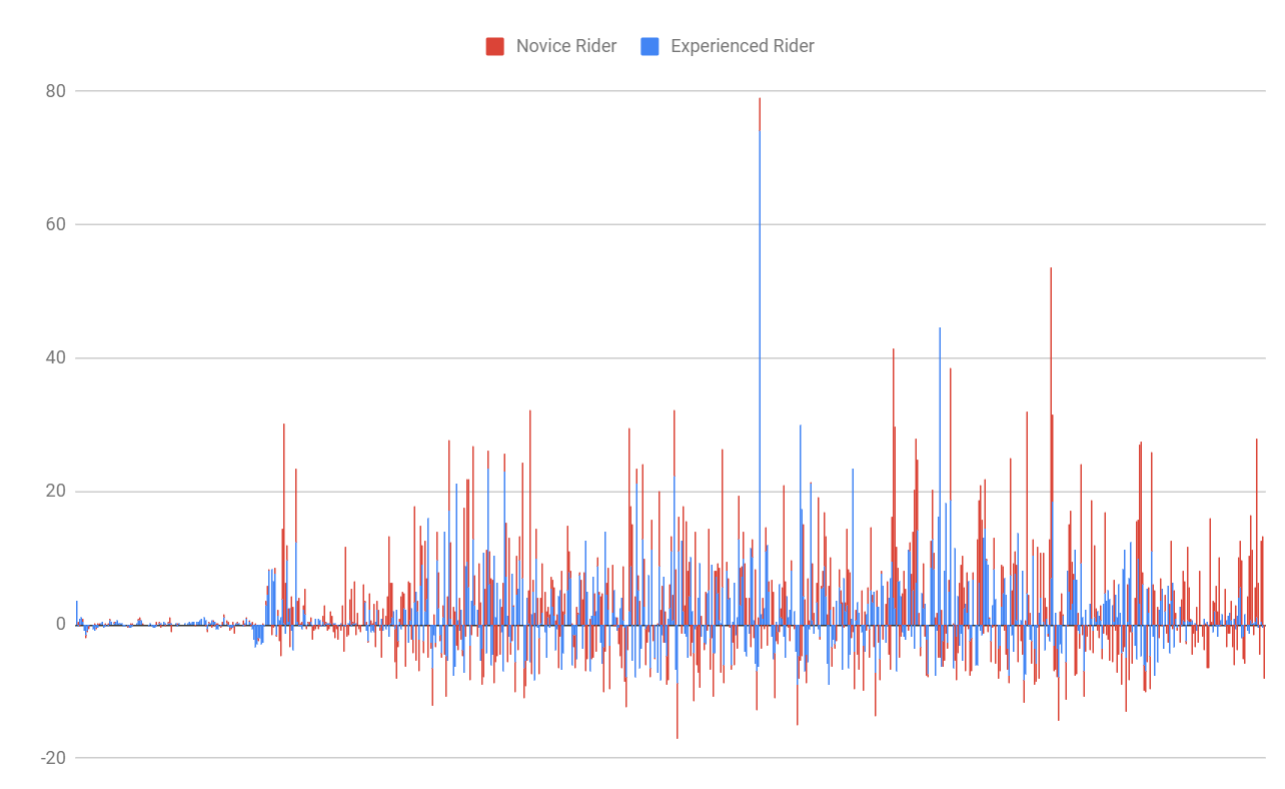
\includegraphics[scale = 1]{background/slowvfast.png}
      \caption{G-Force experienced by two different riders on the same trail}
      \label{forces}
\end{figure}
%%%%%%%%%%%%%%%%%%%%%%%%%%%%%%%%%%%%%%%%




\section{Rule Based Solutions}
An extension of threshold based solutions are rule based solutions, a popular method used in fall detection \cite {commonSolutions} .  Rule based solutions utilize a rulebase as a means of determining if an event has occurred. Analysing raw data allows for feature extraction to which a set of rules can be derived. E. g., if accelerometer reading is greater than threshold AND gyroscope reading is greater than threshold THEN a crash has occurred, a similar premise to the rules used in a mamdani fuzzy inference system.

Rule based solutions allow for more in depth understanding of the event that occured. False positives can be greatly reduced by constructing rules targeted to fire iff the sensor reading align with the signature off a fall, ruling out false positives which would be triggered by ADL similar in nature to a fall. These systems work quite well for medical applications, threshold driven rules are actually quite suitable for slow moving humains moving around a home, very few daily tasks would surpass thresholds set for falling over. The forces experienced during ADL have been shown to be far lower than what is experienced during a fall for instance\cite{smart}.

A review of fall detection methodologies found that the most common implementation consisted of  systems using a combination of threshold and rule based methods combined, 42 out of 51 (82\%) of the existing solutions were rule based using thresholds \cite {commonSolutions}. 



\section {Machine Learning Techniques}
Machine learning techniques are commonly used in the development stages of a system. Using real world test data of known falls or crashes to train the model, the optimal threshold can be computed. For medical applications this is common practice as there isn't a huge variance in fall patterns when one is in the home.  Learning is rarely used in real-time as the low cost, basic hardware isn't capable of running complex algorithms in real-time. Experimental studies have shown the benefits of utilizing a combination of live sensor readings in conjunction with learning techniques, for example 96\% accuracy has been achieved using k-NN \cite{mls} . While Learning can improve accuracy, its complexity makes a simpler solution such as a rule-threshold based solution, a more appealing solution for low cost implementations.

For more advanced systems  the most popular machine learning techniques are Support Vector Machines (SVM), Naïve Bayesian classifiers , k-Nearest Neighbors (k-NN) and binary decision trees. Choosing one method over another is not trivial as results vary to which performs the most accurately for fall detection. Findings from existing studies show no clear winner as the test methodologies differ from study to study producing different results in accuracy. As no one sensor make or model is used accuracy can also be dependant on sensor quality.









